\documentclass[sigconf]{acmart}

\usepackage{graphicx}
\usepackage{hyperref}
\usepackage{todonotes}

\usepackage{endfloat}
\renewcommand{\efloatseparator}{\mbox{}} % no new page between figures

\usepackage{booktabs} % For formal tables

\settopmatter{printacmref=false} % Removes citation information below abstract
\renewcommand\footnotetextcopyrightpermission[1]{} % removes footnote with conference information in first column
\pagestyle{plain} % removes running headers

\newcommand{\TODO}[1]{\todo[inline]{#1}}

\begin{document}
\title{Big Data Applications in Predicting Hospital Readmissions}

\author{Tyler Peterson}
\orcid{1234-5678-9012}
\affiliation{%
  \institution{Indiana University - School of Informatics, Computing, and Engineering}
  \streetaddress{711 N. Park Avenue}
  \city{Bloomington} 
  \state{Indiana} 
  \postcode{47408}
}
\email{typeter@iu.edu}

% The default list of authors is too long for headers}
\renewcommand{\shortauthors}{G. v. Laszewski}

\begin{abstract}

  Hospital readmissions occur when a patient is discharged from a hospital and subsequently readmitted to a hospital within a short time frame. Hospitals are held accountable and penalized for readmissions that occur within 30 days of the initial inpatient stay. In 2016, nearly 2,600 hospitals were penalized \$528 million collectively for readmissions. Machine learning is increasingly being used to build models that predict if a patient has a high probability of being readmitted, which allows hospital staff to prioritize resources around high-risk patients and potentially prevent the otherwise likely readmission. Healthcare providers possess every-growing stores of medical data that are essential for building accurate predictive models. While most of this information is private and not widely available for research, there are a few public datasets that researchers can use to build models and gain a better understand of which information is significant in the task of identifying high-risk patients. One such dataset includes over 100,000 patient admissions that occurred at 130 US hospitals between 1999 and 2008 and includes many features that can be used to build models. Open-source Python tools such as scikit-learn, pandas and matplotlib have tools necessary for preparing, modeling and visualizing data. These tools can be used to define algorithms that describe the problem of hospital readmissions by creating classifiers that categorize patients based on the probability of readmission. Machine learning techniques, such as logistic regression, are capable of modeling data for classification problems, and these tools include methods for assessing and optimizing the algorithms. In this analysis, the model created using logistic regression performed better than random guessing, but not well enough to reasonably be considered a highly effective model. The sensitivity of the model is rather low for a problem where there is a high cost of missing an opportunity to intervene on a patient at high-risk of readmission. The lack of behavioral and social attributes in the dataset may lend to lower predictive power. In any case, the effectiveness of machine learning in classifying patients for risk of readmission is a growing topic of study and implementation of tools for assisting healthcare providers will likely continue to increase.
 
\end{abstract}

\keywords{hid331, i523, Big Data, Hospital Readmissions, Machine Learning, Classification, Python}

\maketitle

\section{Introduction}

Hospital readmissions are problematic for both patients and healthcare providers. Even a single hospital admission for a patient can be an inconvenient, expensive and anxiety-inducing major life event. For a patient to be subsequently readmitted to the hospital, the patient again experiences the negative aspects of being in a hospital, along with a diminished quality of life that accompanies a recurrent disease or medical issue. Healthcare providers are increasingly being held accountable and often penalized for an inability to keep recently discharged patients from being readmitted. It has been estimated that nearly 1 in 5 Medicare patients discharged from a hospital will be readmitted within 30 days \cite{cite05}.

The Hospital Readmission Reduction Program (HRRP), which originated in 2013 as a provision in the Affordable Care Act, serves as an example of an initiative that punishes hospitals for readmissions by administering financial penalties on hospitals with disproportionately high readmission rates among Medicare beneficiaries \cite{cite06}. The HRRP levies a reduction in Medicare reimbursement, and uses the 'all-cause' definition for readmissions, which means that a subsequent hospital stay that occurs for any reason within 30 days of the initial stay counts against the hospital \cite{cite06}. The program focuses on patients initially admitted with a heart attack, heart failure, pneumonia, chronic obstructive pulmonary disease, a coronary artery bypass graft procedure or a hip/knee replacement procedure \cite{cite06}. If a hospital's risk-adjusted readmission rate is higher than the national average, then that hospital will be penalized. Further, the excessiveness of the rate is considered as well, ensuring that providers with the worst readmission rates have proportionately higher penalties \cite{cite06}. In 2016, the US government penalized 79 percent of US hospitals, which amounts to 2,597 institutions \cite{cite00}. The penalties for those readmissions, applied to the 2017 fiscal year reimbursements, amounted to \$528 million nationally, \$108 million higher than the previous year \cite{cite00}.

Effectively this means that the care provided to readmitted patients is uncompensated care, which still requires valuable resources such as medical supplies, pharmaceuticals, the occupancy of hospital beds and the attention of medical staff. HRRP has had the intended effect of bringing increased attention to readmissions, and some healthcare providers are leveraging their ever-increasing medical data stores to better understand their patients. Several organization are using machine learning to identify high-risk patients. Assessing patients for the likelihood of readmission presents a binary classification problem, where a model's goal is to come to one of two conclusions on each case. The model analyzes each patient and the patient's accompanying attributes and concludes either that the patient will be readmitted or will not be readmitted.

\subsection{Applying Machine Learning to Hospital Readmissions}

There are several studies pertaining to the effectiveness of using machine learning to build predictive models that address this problem. A 2011 study conducted a systematic review of the topic and found 26 studies discussing predictive models related to hospital readmissions. These models were created using administrative claims data, electronic medical record (EMR) data, or a combination of each type of dataset \cite{cite08}. Administrative claims data is primarily gathered for billing purposes and contains information about procedures, diagnoses, length of hospital stay and location of care \cite{cite10}. The advantage of this type of data is that it typically describes large populations and is inexpensive to acquire because it's already gathered for billing \cite{cite05}. EMRs contain the basic information contained in adminstrative claims data, and also include lab data, image data and the results of various diagnostic tests, as well as social and behavioral information. Of the 26 studies reviewed by this paper, only 4 reported an area under the curve (AUC) value greater than 0.70, indicating that the other 22 models performed relatively poorly at classifying high-risk patients. Interestingly, 3 of the 4 studies with a moderately high AUC built models with clinical information found in EMRs in addition to administrative claims data, which suggests that the rich information available in EMRs adds discriminative power to the predictive models \cite{cite05}.

One study that demonstrates the power of incorporating EMR data was conducted at Mount Sinai Health System in New York, NY. Mount Sinai developed a model to predict readmissions among patients with heart failure, which is the top cause of readmission among Medicare beneficiaries \cite{cite01}. To build the model, Mount Sinai leveraged their EMR system to mine 4,205 patient attributes, including 1,763 diagnosis codes, 1,028 medications, 846 laboratory measurements, 564 surgical procedures, and 4 types of vital signs. The study used a cohort of 1,068 patients, 178 of whom were readmitted within 30 days \cite{cite01}. The model achieved a prediction accuracy rate of 83.19 percent and an AUC value of 0.78. Commenting on this outcome, Mount Sinai said that the model would benefit from the inclusion of several years of data from several different hospital sites \cite{cite01}. In other words, even more data is needed to further improve the accuracy of the model.

\section{Analysis}

Though the data used by institutions to build models is not widely available, there are a few public datasets that can be used by machine learning practitioners to better understand how predictive modeling techniques can be applied to the task of predicting readmissions. One such dataset comes from from the Cerner Corporation's Health Facts database, which is comprised of comprehensive clinical EMR records voluntarily provided by hospitals across the United States \cite{cite11}.

Researchers extracted a subset of 101,766 encounters from the nearly 74 million records in the Health Facts database for the purpose of studying diabetic inpatient encounters. The admissions span 10 years from 1999 to 2008, and occurred at 130 different hospitals across the United States. The researchers used the following criteria to narrow down the dataset \cite{cite11}:

1) The encounter is an inpatient encounter.

2) It was a diabetic encounter, meaning at least one diabetic diagnosis code was associated with the episode of care.

3) The length of stay was between 1 and 14 days.

4) The patient had at least one lab test.

5) The patient was administered at least one medication.

This dataset is now publicly available on the UCI Machine Learning Repository. Each observation in the dataset has up to 55 attributes, or features, that are potentially related to hospital readmissions, including diagnoses defined by ICD9 codes, in-hospital procedures, hospital characteristics, individual provider information, lab data, pharmacy data, and demographic data, such as age, gender and race. Each patient encounter record also has a label indicating whether or not the patient was readmitted within 30 days. Since the dataset includes these labels, supervised machine learning techniques can be used, as opposed to unsupervised machine learning techniques. Logistic regression is a supervised machine learning technique capable of binary classification of observations, and is well-suited to predict the likelihood of readmission for the observations in this diabetes dataset.

\subsection{Overview of Supervised Machine Learning}

\subsubsection{Minimization of Error}

The goal of a machine learning algorithm is to minimize the error made in the predictions. The general form of this concept can be represented by the formula:

\[Y = f(x) + \epsilon\]

\(Y\) is the actual outcome associated with the sample. \(x\) represents the attributes associated with each sample and typically takes the form of a matrix where the columns are the features and the rows are the individual observations. \(f(x)\) is a function that represents the systematic information \(x\) provides about Y, and \(\epsilon\) is the error term describing the differences between the predicted value returned by \(f(x)\) and the actual value represented by \(Y\) \cite{cite03}. A perfect prediction means \(f(x)\) equals \(Y\) and \(\epsilon\) equals zero. In reality, the error term will rarely be zero, so each prediction yields a certain amount of error. The prediction accuracy for each sample is evaluated by this formula, and sum of the error terms from each evaluation represents the magnitude of error made by the model. The goal is to make the sum of errors as low as possible \cite{cite03}.

The error term is minimized through optimization of \(f(x)\), which is intended to describe the patterns that exist between the independent variables, represented by \(x\), and the dependent variable, represented by \(Y\). Said differently, the equation describes the relationship between the features and the outcome label. The way that this function describes this relationship is through coefficient weights. Each feature in the dataset is paired with a numerical weight that accentuates or diminishes the impact of a feature on the predicted outcome. The way in which these coefficients can be interpreted differs by which algorithm is used, but the intuition remains the same: the coefficients are adjusted to highlight the important features in the dataset. Once the coefficients are determined, the model has been fit to the data.

\subsubsection{Training Set vs. Test Set}

The coefficient weights of the model are defined by analyzing the samples in a dataset. In a practical sense, the value of a model depends on its ability to accurately predict the outcomes of new samples that were unseen at the time the model was determined \cite{cite08}. A model that performs well when making predictions with new data is said to generalize well.
A machine learning practitioner will want to have confidence in the model's ability to generalize before deploying the model to make predictions in real-time, and will not necessarily have a new dataset of previously unseen observations to run through the model. To get around this, the original dataset is often split into two parts. The first part of the dataset is referred to as the training set and is used to determine the coefficient weights. The second part of the dataset is referred to as the test set, and this set is run through the model derived from the training set. The accuracy of the predictions on the test set is compared to the accuracy of the predictions on the training set to determine the extent to which the model generalizes \cite{cite08}.
A model that has high training accuracy, but low test accuracy, is said to be overfitting the data. This means that the model, in its efforts to minimize \(\epsilon\), has become too complex and focuses too closely on the samples in the training dataset. By chasing patterns in the training data caused more so by random chance than by the true characteristics of \(x\), the model no longer generalizes to the unseen samples in the test set \cite{cite03}\cite{cite08}. An overfit model describes characteristics in the training data that are not in the test data, leading to poor predictions on the test set.
A model can also underfit the data, which means the model is failing to capture the relationship between \(Y\) and \(x\) and will likely perform poorly on both the training and test datasets.

\subsubsection{The Bias/Variance Trade-off}

Bias and Variance are two important components related to training models using machine learning. Variance describes the extent to which a model changes due to small adjustments in the training data. Since the training data used to fit a model can vary, it is reasonable to expect that a model will change when different samples are selected into the training dataset, but ideally the model changes only slightly \cite{cite03}. If a model is quite complex and is overfitting the training data, then slight changes in the training samples can have a large effect on the coefficient weights. Low variance is preferable \cite{cite03}.

Bias refers to the error that occurs when trying to describe a phenomenon using a model. For example, if a machine learning technique assumes a linear relationship between the independent and dependent variables, but the relationship is highly non-linear, then the model has high bias \cite{cite03}. A model with high bias will make many erroneous predictions because the estimated relationship between \(x\) and \(Y\) is not closely aligned with the actual relationship between \(x\) and \(Y\).

As a model becomes more complex and able to fit to the perceived important information in the training data, variance will increase and bias will decrease. The model will become more flexible and therefore more sensitive to variations in the training data, but will reduce bias by better estimation of the relationship between \(x\) and \(Y\), resulting in a reduction in the prediction error. The important part of the relationship between these two components is that as a model becomes more complex, the bias decreases more rapidly than the variance increases, so the trade-off of increasing variance while decreasing bias leads to a net gain in improvement of the model \cite{cite03}. However, there is a point at which the model becomes too complex and the net gain begins to disappear. Increased model complexity leads to significantly higher variance without appreciable improvement in bias \cite{cite03}. 

\subsubsection{Model Evaluation}

Several statistics can be used for evaluating model accuracy. For classification problems, a basic technique for evaluation is the confusion matrix.

\[ 
\left \{
  \begin{tabular}{ccc}
  TN & FP \\
  FN & TP 
  \end{tabular}
\right \}
\]

This is the general framework of a confusion matrix which shows the counts of each type of prediction and the accuracy of that prediciton. A true positive (TP) is an outcome that is predicted to be positive and is positive in reality \cite{cite12}. A true negative (TN) is an outcome that is predicted to be negative and is negative in reality \cite{cite12}. These are the preferred responses. In the context of hospital readmissions, a true positive is a prediction that a patient in the test dataset, according to the trained model, will be readmitted to the hospital within 30 days, and this occurs in reality. A true negative is a prediction that a patient in the test dataset will not be readmitted, and this occurs in reality.

On the other hand, a false positive (FP) is an outcome that is predicted to be positive but is negative in reality \cite{cite12}. A false negative (FN) is an outcome that is predicted to be negative but is positive in reality. These are errors in prediction \cite{cite12}. If a healthcare provider acts on a false positive, that could mean that a patient, who without intervention would not have been readmitted within 30 days, received resources and attention that were not necessary. In the case of a false negative, this means a patient who eventually did get readmitted within 30 days, but was said to be of low-risk of readmission, could have benefited from additional attention and resources from a healthcare team.

These four components - true positives, true negative, false positives, and false negatives - can be combined to create more nuanced metrics. Two of those metrics are sensitivity and specificity. Sensitivity refers to the true positive detection rate. This is the percentage of positive occurrences that are successfully identified \cite{cite12}. Specificity is the true negative detection rate. This is the percentage of negative occurrences that are successfully identified \cite{cite12}.

In the context of readmissions, low sensitivity means many patients who eventually get readmitted are not predicted to be high-risk before the readmission occurs. Low specifity means that many patients who would not otherwise be readmitted are predicted to be readmitted. There is a trade-off between sensitivity and specificity, and an improvement in one often causes the other to worsen. Preference toward sensitivity or specificity often depends on the cost of incorrect predictions.

A patient who otherwise would not be readmitted who is predicted to be high-risk is the type of case that will incur unnecessary resources. While this requires healthcare providers to invest resources that are not needed, the readmission is nevertheless avoided and there are potentially other benefits achieved by the hospital, such as increased satisfaction of the patient and their family. On the other hand, a patient who eventually gets readmitted but was not identified beforehand will likely be costly to a hospital in a couple ways. The provider must dedicate resources to stabilizing and healing the patient, while also incurring penalties if this type of readmission occurs frequently. If the expense of an unexpected readmission is higher than the expense of deploying unncecessary resources to low-risk patients, then a model that favors higher sensitivity at the expense of lower specificity is preferable.

Sensitivity and specificity can be assessed in tandem by the receiver operating characteristic (ROC) curve, which is quite useful for evaluating supervised classification models. The ROC curve plots the true positive rate against the false positive rate (100 minus the true negative rate) for varying decision thresholds. This illustrates the trade-off between sensitivity and specificity and can provide guidance on which decision threshold is appropirate for the task \cite{cite12}. ROC curves are often leveraged to evaluate the performance of models by calculating the area under the ROC curve, also known as the AUC. The goal is the maximize the AUC value, and that value points to the optimal balance between sensitivity and specificity \cite{cite12}.

\subsection{Logistic Regression}

\subsubsection{Logistic Regression - Intuition}

Logistic regression models the probability that a sample belongs to a certain class given the feature values of the sample \cite{cite08}. This probability can be represented as:

\[p(x) = Pr(Y = 1 | X)\]

In the context of predicting hospital readmissions, this translates to the likelihood that a patient will be readmitted within 30 days of discharge given the patient's characteristics. To determine the probability, logistic regression utilizes the logistic function, which takes in the coefficient weights and feature responses for each sample and returns a the probability - a number between 0 and 1 \cite{cite08}. In the case of logistic regression involving multiple features, the model takes the form:

\[ f(x) =\frac{e^{\beta_0 + \beta_1X_1 + ... + \beta_pX_p}}{1 + e^{\beta_0 + \beta_1X_1 + ... + \beta_pX_p}}  \]

The model is fit to the data by adjusting the coefficient weights using a method called maximum likelihood. The intuition of this process is that the estimates for the coefficients are set such that the predicted probability of a certain outcome corresponds as closely as possible to the actual label of that sample. This means that the ideal coefficient weights, when plugged into the logistic function, return a number close to one for the readmitted patients and a number close to zero for the patients not readmitted \cite{cite08}.

\subsubsection{Logistic Regression - Data Pre-processing}

Data often need to be processed prior to using logistic regression because this machine learning technique requires numerical data. The diabetes dataset contains a combination of continuous and categorical features. For example, 'num\_procedures' and 'num\_lab\_procedures' are continuous features that describe the number of procedures and the number of lab procedures, respectively. Since these columns already contain numerical data, these features are ready to use as-is. Other columns such as 'A1Cresult' includes values such as 'A1Cresult\_$>$7', 'A1Cresult\_$>$8', 'A1Cresult\_None' and 'A1Cresult\_Norm'. The first issue is that this features is represented by text values, which will not work with logistic regression. These values must be encoded to work properly. If a categorical feature with four unique values, or levels, has an ordinal scale, the text values can be encoded as sequential numbers, such as 1, 2, 3 and 4. If a categorical features with four levels has a nominal scale, as is the case with the feature 'A1Cresult', an effective encoding strategy is to create one dummy column for each level in the original categorical column.

The Python library pandas has a function called 'get\_dummies' that will create one column for each level in a categorical column, and each of those dummy columns will only contain 0's and 1's. In the case of the column 'A1Cresult', this process will yield 4 columns. For each observation, a 1 will appear in the column corresponding to the value of the original feature. For example, if an observation had a value of 'A1Cresult\_$>$7', the observation will have a 1 in the 'A1Cresult\_$>$7' dummy column and 0's in the other three A1C dummy columns. This process is repeated for all nominal categorical variables.

Three categorical columns in the dataset have several hundred unique values, which can be problematic. The columns 'diag\_1','diag\_2' and 'diag\_3' have 695, 724 and 757 unique values describing ICD9 diagnosis codes, respectively. The first diagnosis column is considered to be the primary diagnosis of the stay, and 'diag\_2' and 'diag\_3' contain any additional diagnoses documented during the stay. Running these columns through the 'get\_dummies' procedure would yield a total of 2,176 dummy columns, which would greatly increase the dimensionality of the dataset. Further, many ICD9 codes are used only a few times in the dataset, which means it is quite likely that, depending on how the training and test data is split, all observations of a particular code only fall in either the training set or the test set.

One solution to this problem is to 'bin' the information into categories. Each ICD9 code belongs to a category. For example, ICD9 code '250.62 - Diabetes with neurological manifestations, Type II, uncontrolled' is in the ICD9 category 'Endocrine, Nutritional, Metabolic, Immunity'. Each ICD9 code can be binned into one of 19 categories. Further, instead of having three columns for each ICD9 category (because each unique ICD9 code can appear in any of the three diagnosis columns), the data can be processed such that there is one column for each ICD9 category, and each observation can have up to three 1's in these 19 dummy columns. This loses the distinction between primary and secondary diagnoses, but reduces computation time and reduces the likelihood of the rare diagnosis codes only appearing in the test set or training set.

Another column in the dataset called 'medical\_specialty' has a high number of unique values with 71 different responses, and also is null in nearly half of the observations. Rather than turning this feature into 71 different dummy variable columns, it is noted that there is redundancy between the 'medical\_specialty' and the diagnosis code columns. For example, if a patient has a diagnosis code in the 'Pregnancy, Childbirth, and the Puerperium' category, they are often in the obstetrics medical specialty. Given this redundancy, the high percentage of null values and in the interest of reducing the complexity of the dataset, the 'medical\_specialty' column is not included in the final dataset.

Several patients have multiple observations captured in the dataset. Logistic regression requires that the observations be independent, so including multiple inpatient encounter for individual patients violates this requirements. To solve this problem, the inital count of 101,766 observations is reduced down to 69,988 observations by keeping only the first encounter for each 'patient\_nbr'. The first encounter per patient is considered to be the observation with the lowest 'encounter\_id', which operates on the assumption that IDs are incremented by 1 and allocated sequentially as inpatient admissions occur.

Lastly, the response label in the original dataset is represented with three levels and is described in text. The column 'readmitted' contain the values 'NO', '$>$30' and '$<$30'. Since observations with the label '$>$30' days were not readmitted within thirty days, these labels were converted to 'NO'. The remaining responses of 'NO' and '$<$30' were encoded as 0 and 1, respectively.

\subsubsection{Logistic Regression - Data Quality Evaluation}

When creating dummy columns, whether through simple methods, such as the 'A1Cresult' transformation, or more complex methods, such as the ICD9 diagnosis binning transformation, special consideration must be given to collinearity and multicollinearity between features. For example, if a feature called 'gender' contains two values, male and female, and this feature is converted into two dummy features, these two features will be collinear. Where one feature column has a value of one, the other will have a zero, and visa versa. This means that one feature column can perfectly predict the value of the other feature column. We only need the female column to know if the observation pertains to a male or female, so the inclusion of the male column would be redundant. This is problematic for the model because the two feature columns provide an identical explanation of the variance in the dependent variable, and neither adds additional value while in the presence of the other. When this issue manifests between two columns, this means the columns are collinear. Multicollinearity refers to a situation where this redundancy occurs between three or more columns. If the combination of three columns explains most of the variation explained by another single column, then there is multicollinearity in the data.

Collinearity and multicollinearity increase the variance of the coefficient weights, which would make the model very sensitive to changes in the training data. This instability of the weights means that it can be difficult to decide which predictors have a high influence on the outcome, and can even cause the sign of the coefficient to change \cite{cite16}. Under stable conditions, a positive coefficient can be interpreted to mean that the associated feature contributes to a higher probability of readmission, and a negative coefficient can be interpreted to mean that the associated feature contributes to a low probability of readmission \cite{cite03}. The instability that multicollinearity creates in the coefficient weights make it dubious to make inferences from the signs of the weights.

Datasets with collinearity and multicollinearity issues are considered to be ill-conditioned, which will reduce the ability to create a meaningful model with the data. Problematic features need to be strategically identified and removed. A dataset can be evaluated for problems using several linear algebra methods. The matrix rank is a single value that can give an overall assessment of the relationship between features. In a dataset, which can be represented as a matrix, that has more rows than columns, the ideal matrix rank value is equal to the number of columns. When the matrix rank value is equal to the number of columns this means the matrix is considered to be full rank \cite{cite14}. A full rank matrix contains only linearly independent features. On the other hand, if a feature in a dataset is linearly dependent, then the rank of the matrix is reduced. For example, if we were to keep both the male and female gender dummy columns, these features would be considered linearly dependent, and would therefore reduce the rank of the matrix. Each linearly dependent feature in a dataset reduces the matrix rank.

A correlation matrix provides a correlation statistic for each pair of variables. The values fall between -1 and 1, and the closer the value is to -1 or 1, the stronger the relationship between the two variabeles. Features with high correlation are considered to be collinear. This technique is effective at finding collinearity, but is not well-suited to finding multicollinearity because the correlation matrix only shows the relationship between pairs of variables.

The correlation matrix can also be used to find the determinant of the dataset. The determinant is a single value and  will reveal if there are any highly or perfectly correlated columns, which suggests there is collinearity among features. The determinant value ranges between 0 and 1. A value of zero means the correlation matrix is singular. In other words, the correlation matrix contains at least one pair of perfectly correlated features. A near-zero determinant value means there is one or more pair of features that is nearly correlated. A higher determinant value is preferable.

These methods are effective at describing the overall health of the dataset and simple relationships between pairs of features. To find multicollinearity, more nuanced techniques need to be deployed. One approach is to determine the variance inflation factor (VIF) for each independent variable. The VIF measures the increase of variance in the coefficient estimates that is caused by the inclusion of a particular variable \cite{cite15}. This technique fits each independent variable, one at a time, against all of the other independent variables. This can be represented by the following sequence of equations:

\[X_1 = \beta_2X_2 + \beta_3X_3 + \beta_4X_4 + ... + \beta_kX_k \]
\[X_2 = \beta_1X_1 + \beta_3X_3 + \beta_4X_4 + ... + \beta_kX_k \]
\[X_3 = \beta_1X_1 + \beta_2X_2 + \beta_4X_4 + ... + \beta_kX_k \]
\[...\]
\[X_k = \beta_1X_1 + \beta_2X_2 + \beta_3X_3 + ... + \beta_{k-1}X_{k-1} \]

For a dataset with k-features, the dataset is fit k-times, once for each independent feature. The VIF for each feature is calculated by the equation:

\[ VIF_k =\frac{1}{1 - R^2_k}\]

Each fitted model has an \(R^2\), which is the coefficient of determination, or R-squared, and it describes the proportion of variation in the 'dependent' variable that is described by the independent variables. A high R-squared means that the independent variables explain a significant amount of variation in the dependent variable. In the context of VIF, if one independent variable is thoroughly explained by the other independent variables, the R-squared will be high which will lead to a high VIF. While the threshold for acceptable VIF values differs, the documentation for the Python library statsmodels recommends using a threshold of 5 \cite{cite15}. To achieve a value of 5 or less, the \(R^2\) for an independent variable must 0.80 or less. In other words, the independent variable being considered by the VIF method must be less than 80\% explained by the other independent variables.

The elimination of problematic variables in this dataset is handled by a custom Python function that identifies the features with the highest VIF and selectively removes those features from the dataset. The Python functions works by calculating the VIF for each independent variable. It then iterates through each group of dummy columns that stemmed from a single categorical column, and, for each group, deletes the column with the highest VIF value if that value is above the threshold. The function also removes ratio-scaled features, such as 'num\_procedures', that have a high VIF value. This whole process is looped until zero features have a VIF above the threshold.

Before trimming features based on VIF, the dataset included 175 features, with a matrix rank of 150 and a correlation matrix determinant of zero, meaning the coefficient matrix was singular. This means there were several linearly dependent features and at least one pair of perfectly correlated features. After trimming 52 features based on VIF, the dataset includes 123 features with a full rank of 123 and a correlation matrix determinant of 0.00697. While this determinant value is still relatively low, the determinant increased over each iteration of the Python function from 0.0 to 2.85e-26 to 0.0056 to 0.00697, representing several orders of magnitude in improvement from the originally singular matrix. Most importantly, the matrix now has full rank with 0 linearly dependent features.

\subsubsection{Logistic Regression - Feature Selection}

With the issue related to multicollinearity among the independent variables largely resolved, the coefficient weights of the model will be more stable, allowing for inferences to be made based on the sign and magnitude of the weights. The next step is to strategically choose which features to use when training the model. Recursive feature selection (RFE) is one strategy for choosing which features have the highest significance in predicting the likelihood of readmission within 30 days. The intuition behind RFE is that it repeatedly fits the model on the training data. The first iteration includes all features, and each subsequent fitting of the data drops the least significant feature or features from the previous iteration. Python has a library called scikit-learn which includes tools to execute RFE on a dataset. The user may choose how many features to trim after each iteration, as well as choose how many features the final model should have. The process will repeatedly fit the narrowing set of features to the data until the preferred number of the most important features is reached.

There is an extension of RFE called RFECV, which helps to determine the ideal number of features. When using RFE on its own, the user must arbitrarily choose the preferred number of procedures. RFECV functions by calculating the accuracy of the model after each iteration of trimming features and re-fitting the model. The number of features used at the step in which the model performance is best is determined to be the ideal number of features to use. The 'transform' method of RFECV will then trim down the original dataset to the selected features. After running RFECV on the remaining 123 features, the process selected 57 features that led to the highest accuracy rate. 

\subsubsection{Logistic Regression - Execute Analysis}

The set of independent variables is trimmed down further to the 57 features selected by RFECV as being the most important for predicting likelihood of readmission within 30 days. The next step is to train the logistic regression model, and then test the accuracy of the model. Scikit-learn has a function that randomly splits the dataset into training and test sets, and also allows the user to decide the size of the test dataset in terms of proportion of overall data. After splitting the features and labels into training and test sets, the data is ready for fitting.

Scikit-learn also has a process for executing logistic regression, and there is a parameter that controls the way the algorithm minimizes coefficients. The default setting is L2 regularization, which determines coefficients that can approach zero (meaning the associated feature does not have a large effect on the outcome) but never fully reach zero. This regularization of coefficients effectively determines how much effect each feature has on the prediction. The less significant features will have a coefficient close to zero. L1 regularization is another option, which sets the less significant features to exactly zero, which can be viewed as another form of feature selection \cite{cite08}.

There is another parameter called C, which dictates the strength of the regularization. Higher values of C lead to less regularization. This means that a model trained with a high value of C will value fitting each observation as closely as possible, whereas a lower value of C will train the model in a way that tries to fit the data more generally \cite{cite08}. A high value of C will lead to higher weight values, and a low value of C will lead to weights that are much closer to zero.

\subsubsection{Logistic Regression - Evaluate Analysis}

The model is trained using both L1 and L2 regularization, and each regularization type is fit using three different values for C: 0.01, 1.0 and 100.0. Figure \ref{f:weightsl2} shows the coefficient weights using L2 regularization and the three different values of C. It is evident that higher values of C lead to larger weights. Figure \ref{f:weightsl1} show the coefficient weights using L1 regularization, again with the different values of C. In addition to the observation that higher value of C lead to larger weights, it is also interesting to note that using 0.01 for the value of C sets all but four weights equal to zero. The four features chosen by this model are the numbers of inpatient encounters, age 50-60, transferred to a skilled nursing facility and discharged to another rehabilitation facility. This pair of L1 regularization and 0.01 for C has the highest training and test set accuracy. The training accuracy is 91.063\% and the test accuracy rate is 90.0827\%. In the original dataset of the 69,998 observations, 63,704 were not readmitted. This is a rate of 91.02\%. This is only slightly smaller than the training accuracy and larger than the test accuracy, which means the model performs closely to the rate that would be achieved if a person guessed that every case would not be readmitted.
The confusion matrix for L1, C = 0.01 model is:

\[ 
\left \{
  \begin{tabular}{ccc}
  12713 & 2 \\
  1282 & 1 
  \end{tabular}
\right \}
\]

12,713 true negatives were identified and 1 true positive, for a total of 12,714 accurate predictions. There were 2 false positives and 1,282 false negatives. The model is effective at predicting patients who will not be readmitted, but the high number of false negatives, compared to the extremely low count of true negatives, demonstrates that the model is not performing well at identifying patients who eventually get readmitted. The models with C values of 1.0 and 100.0 have a true negative detection count of 4, slightly higher than the 1 observation classified correctly by the L1, C = 0.01 model.

The relationship between the true positive and false positive rates can be visualized with an ROC curve. Figure \ref{f:roccurve001} show the ROC curve for the L1, C = 0.01 model. The black dotted line represents the 50/50 chance curve, which is equivalent with guessing. The ROC curve extends slightly above the 50/50 chance curve, which means the predictive power is slightly higher than random guessing. This is described by the AUC, which has a value of 0.50013. This is consistent with the conclusion that model is only slightly better than chance. Figure \ref{f:roccurve100} shows the ROC curve for the L1, 100 model, and the ROC curve bends further away from the 50/50 chance curve, and the AUC is slightly higher at 0.5013. This is consistent with the observation that the model with the higher value of C has a higher true negative detection rate. Ideally, the ROC curve is as close to the upper left hand corner as possible, which would represent a high true positive rate with a low false positive rate.

\section{Conclusion}

The predictive power of the logistic regression model chosen for this analysis appears to be slightly better than random guessing, but not significantly better. The high proportion of false negatives means many patients who are at hish risk of readmission within 30 days, and later get readmitted, are not being identified by the model. This is a domain where high sensitivity is favored over high specificity, but the model conversely has low sensitivity and high specificity. To improve the predictive power of the model, it might be helpful to include features that have more to do with behavioral and social characteristics, as well as socioeconomic indicators. Attributes such as literacy, obesity, annual income, smoking status, medication regimen adherence, utilization of family and community support and employment status are a few features that come to mind that may lend to better explaining the likelihood of readmission within thirty days. Features of this type may help describe the extent to which a patient is able to manage his or her own care outside of the hospital. Patients who cannot read or who do not adhere to the recommended medication regimen, for example, are patients who can reasonably be said to be less capable of providing consistent and effective care to themselves in the home setting. Attributes such as this are not available in the dataset, but common sense suggests this information would be helpful.

Further, logistic regression is just one type of machine learning technique capable of performing classification. Support vector machines and decision trees are two other techniques that would be worth exploring to see if modeling the data using different machine learning algorithms improves the sensitivity of the model.

\appendix

\section{Accompanying Jupyter Notebook and Requirements}
The accompanying Jupyter Notebook is available at: \url{https://github.com/bigdata-i523/hid331/blob/master/project/project.ipynb}

The requirement file is available at: \url{https://github.com/bigdata-i523/hid331/blob/master/project/requirements.txt}

\begin{acks}

The author would like to thank Dr. Gregor von Laszewski and his teaching assistants for their support throughout the semester.

\end{acks}

\bibliographystyle{ACM-Reference-Format}
\bibliography{report}

\section{figures}

\begin{figure}[!ht]
  \centering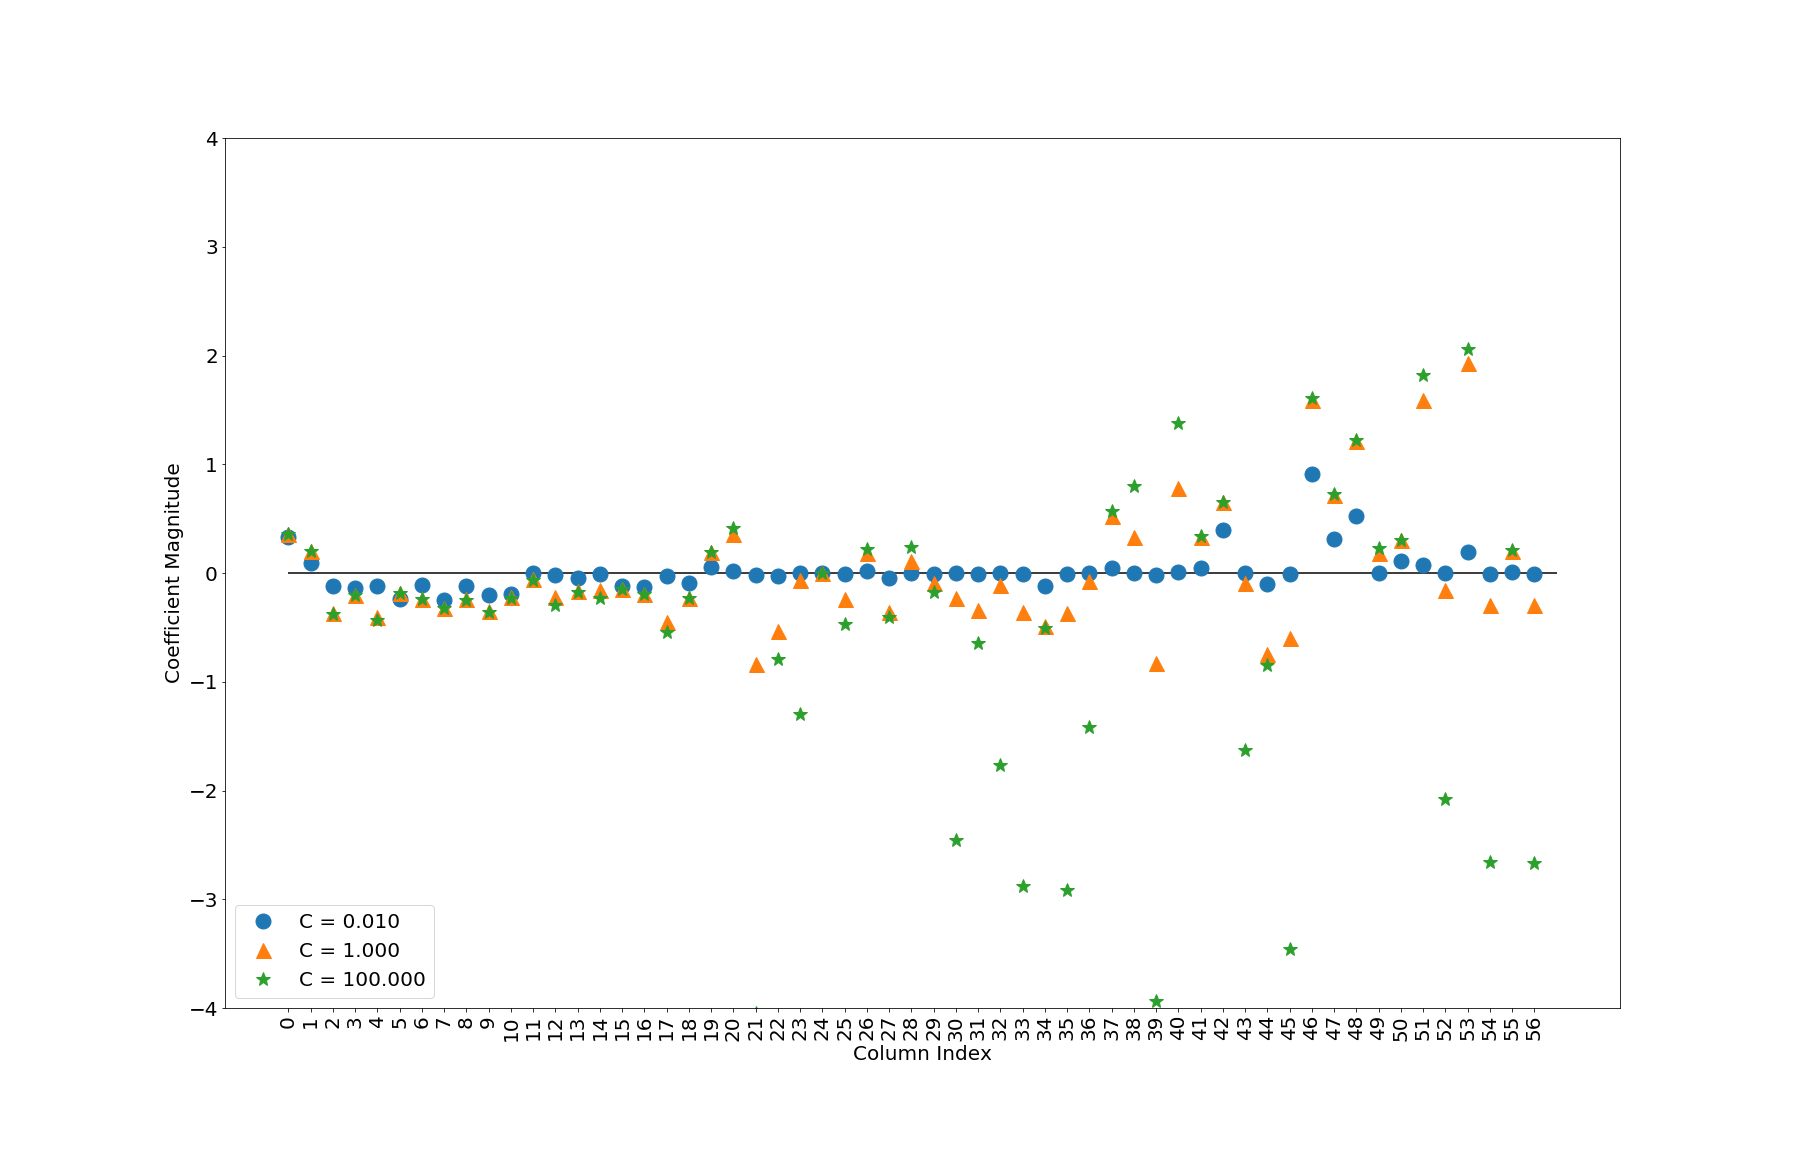
\includegraphics[width=\columnwidth]{images/weightsl2.png}
  \caption{Logistic Regression Weights By C-Value, L2 Regularization}\label{f:weightsl2}
\end{figure}

\begin{figure}[!ht]
  \centering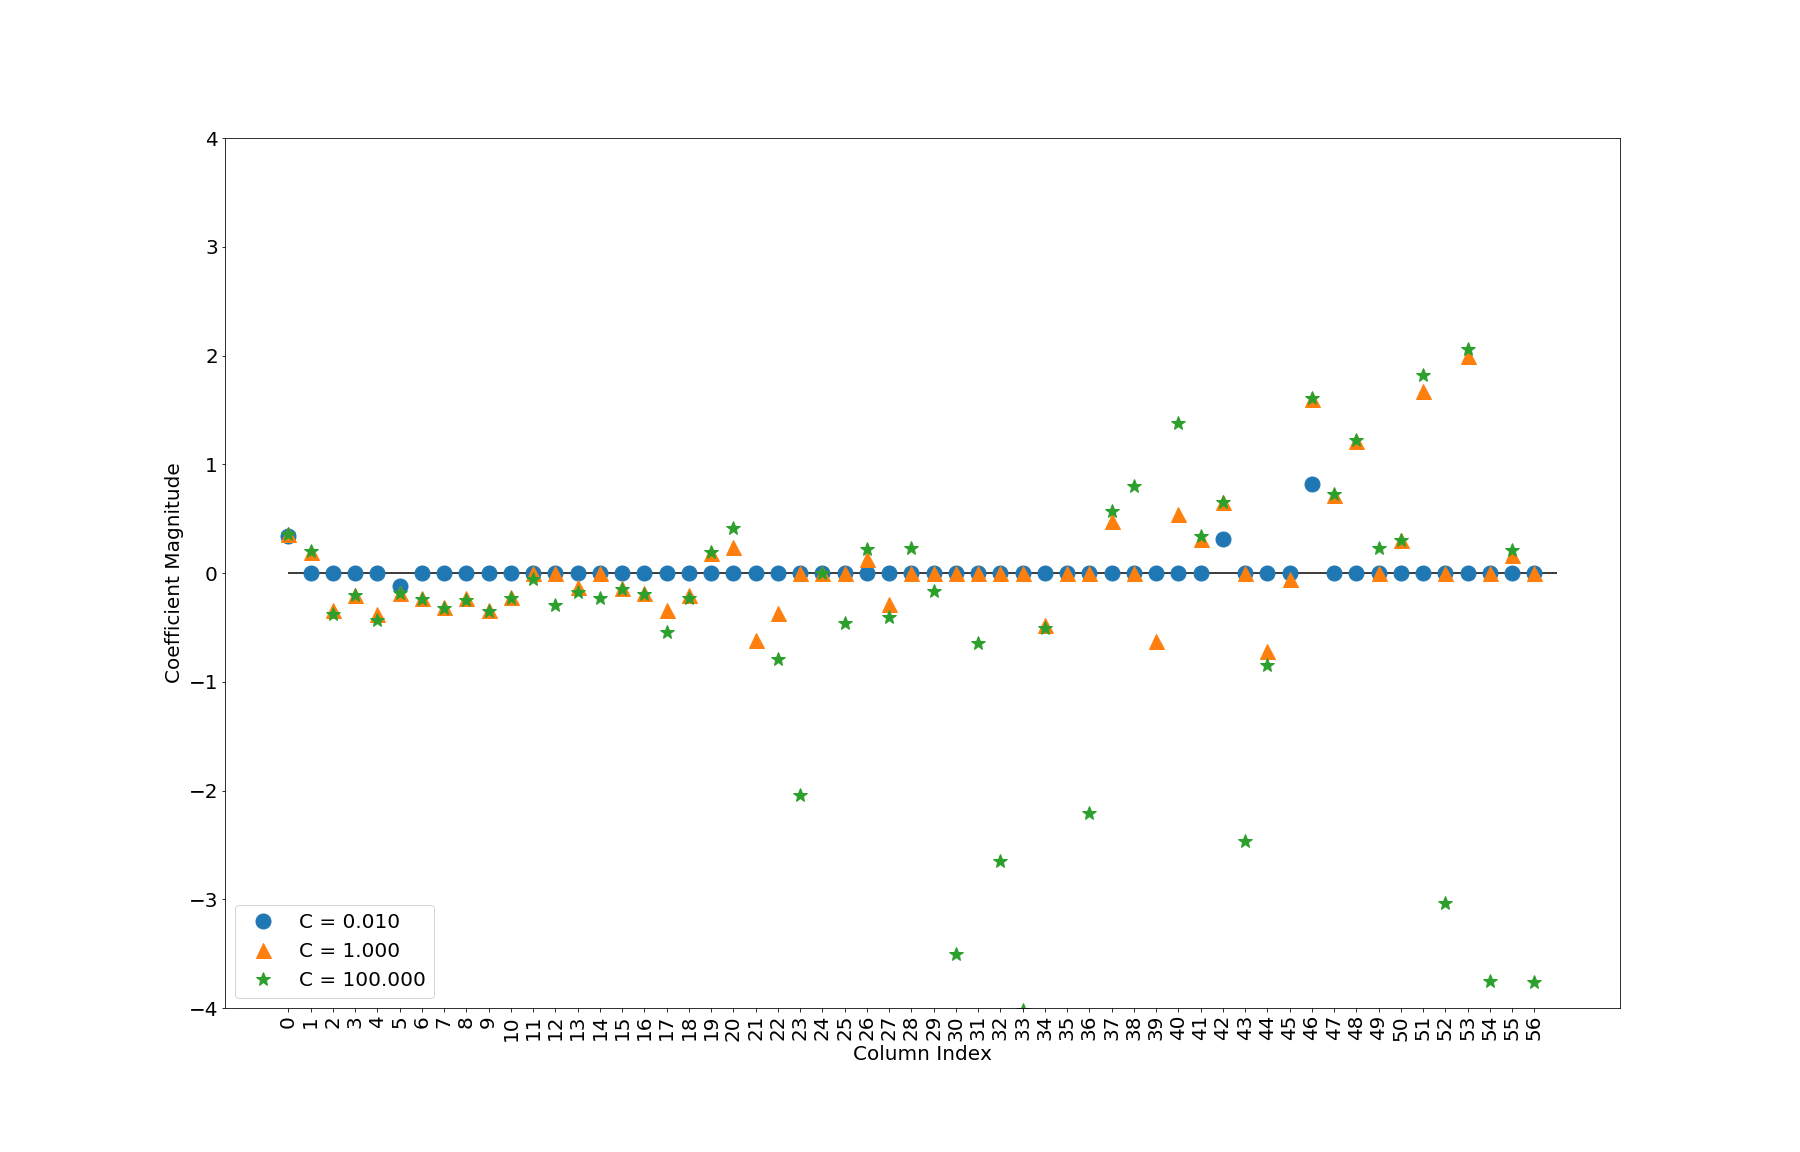
\includegraphics[width=\columnwidth]{images/weightsl1.png}
  \caption{Logistic Regression Weights By C-Value, L1 Regularization}\label{f:weightsl1}
\end{figure}

\begin{figure}[!ht]
  \centering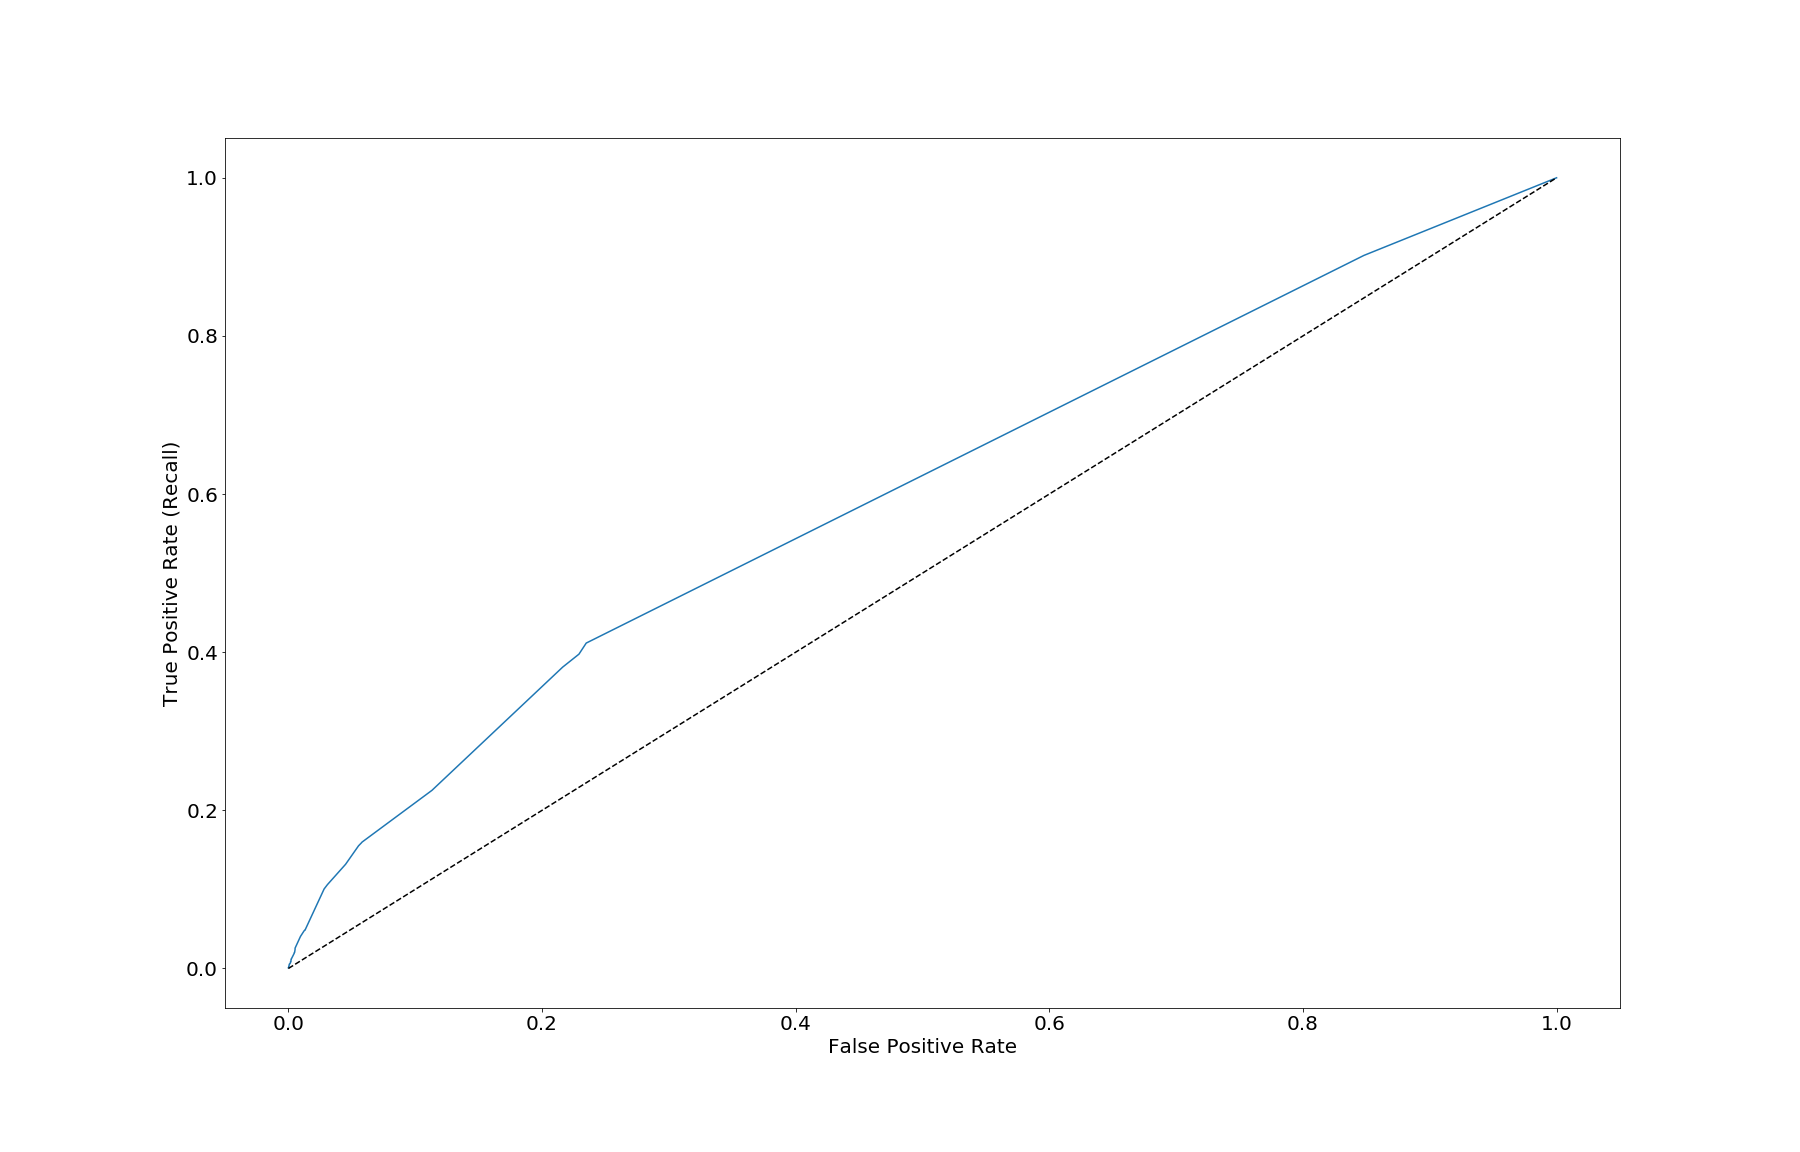
\includegraphics[width=\columnwidth]{images/roccurve001.png}
  \caption{ROC Curve, L1 Regularization, C = 0.01}\label{f:roccurve001}
\end{figure}

\begin{figure}[!ht]
  \centering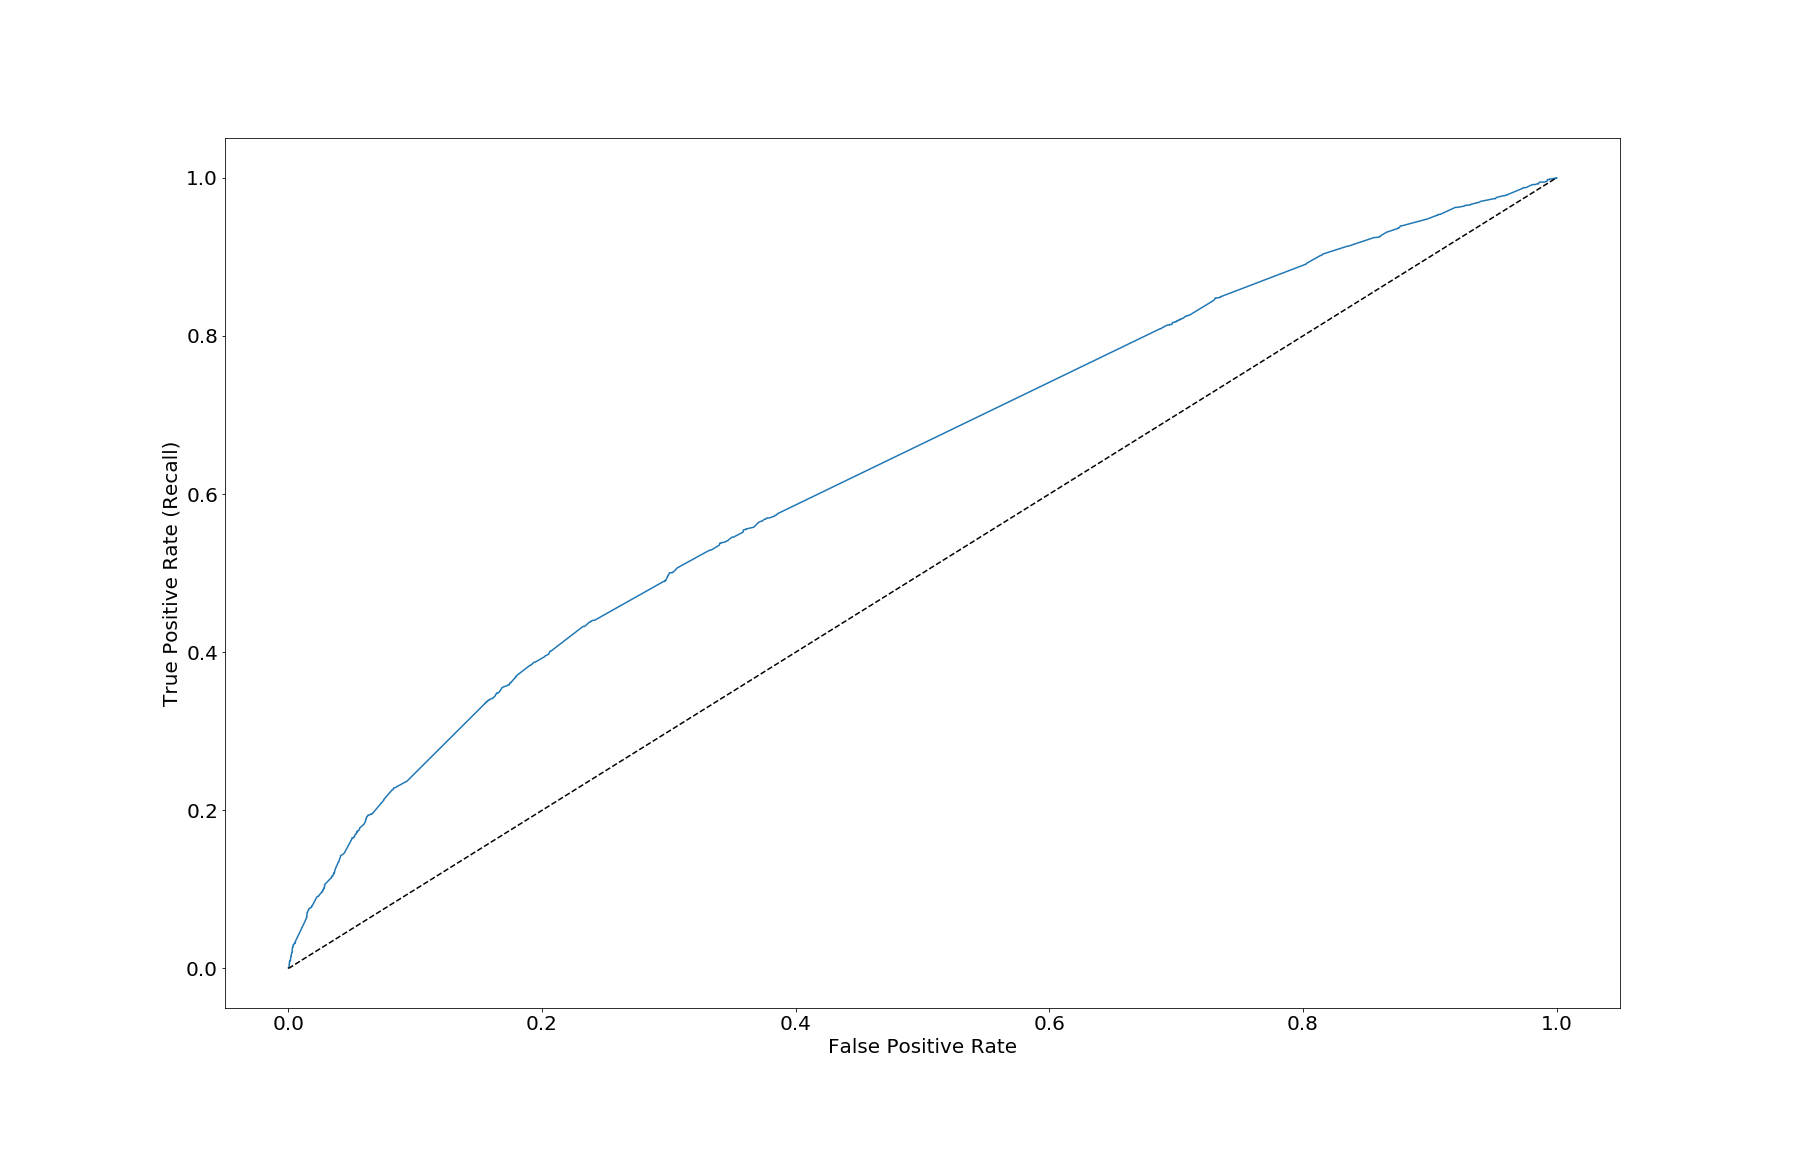
\includegraphics[width=\columnwidth]{images/roccurve100.png}
  \caption{ROC Curve, L1 Regularization, C = 100.0}\label{f:roccurve100}
\end{figure}


\end{document}
